\documentclass[12pt,aspectratio=169]{beamer}

% Input
\usepackage[utf8]{inputenc}
\usepackage[T1]{fontenc}
\usepackage[letterspace=100]{microtype}
\usepackage{upquote}

% Beamer
\usetheme{metropolis}
\usepackage[sfdefault]{FiraSans}
\usepackage{xcolor}
\definecolor{blue}{HTML}{002957}
\definecolor{red}{HTML}{F1563F}
\setbeamercolor{palette primary}{fg=white,bg=blue}
\setbeamercolor{title separator}{fg=red,bg=blue}
\setbeamercolor{frametitle}{fg=white,bg=blue}
\setbeamercolor{progress bar}{fg=red,bg=blue}
\setbeamercolor{alerted text}{fg=red,bg=blue}
\makeatletter
\setlength{\metropolis@titleseparator@linewidth}{2pt}
\setlength{\metropolis@progressonsectionpage@linewidth}{2pt}
\setlength{\metropolis@progressinheadfoot@linewidth}{2pt}
\makeatother

% Graphics
\usepackage{graphicx}
\usepackage{epstopdf}
\DeclareGraphicsExtensions{.png,.pdf,.eps}
\tikzset{
  invisible/.style={opacity=0},
  visible on/.style={alt={#1{}{invisible}}},
  alt/.code args={<#1>#2#3}{%
    \alt<#1>{\pgfkeysalso{#2}}{\pgfkeysalso{#3}} % \pgfkeysalso doesn't change the path
  },
}
\usetikzlibrary{arrows, shapes}

% Various
\usepackage{hyperref}
\usepackage{minted}
\usepackage{fontawesome}
\usepackage{multicol}
\usepackage[normalem]{ulem}

% Title
\title{Deploying Plone and Volto – the Hard Way}
\subtitle{Plone Conference 2020}
\date{9.12.2020}
\author{Asko Soukka}
\institute{\vspace{-0.5cm}
\includegraphics[height=1.5cm]{images/jyu-vaaka-kaksikielinen.eps}\vspace{-0.5cm}\hfill
\includegraphics[width=0.20\paperwidth]{images/nix-snowflake.eps}\raisebox{0.06\paperwidth}{\fontsize{40}{40}\selectfont~+~}\raisebox{-0.5cm}{
\includegraphics[width=0.20\paperwidth]{images/nomad.eps}}}

\newcommand{\setmytemplate}{\usebackgroundtemplate{\begin{picture}(0,0)(-5,250)\footnotesize\href{https://twitter.com/datakurre}{\faTwitter~datakurre}\end{picture}\begin{picture}(0,0)(-330,298)
\includegraphics[width=0.40\paperwidth]{images/plone-icon.pdf}\end{picture}}}

\newcommand{\setnixtemplate}{\usebackgroundtemplate{\begin{picture}(0,0)(-5,250)\footnotesize\href{https://twitter.com/datakurre}{\faTwitter~datakurre} \end{picture}\begin{picture}(0,0)(-355,320)
\includegraphics[width=0.40\paperwidth]{images/nix-snowflake.eps}\end{picture}}}

\newcommand{\setnomadtemplate}{\usebackgroundtemplate{\begin{picture}(0,0)(-5,250)\footnotesize\href{https://twitter.com/datakurre}{\faTwitter~datakurre}\end{picture}\begin{picture}(0,0)(-335,340)
\includegraphics[width=0.40\paperwidth]{images/nomad.eps}\end{picture}}}


\newcommand\Wider[2][1cm]{%
\makebox[\linewidth][c]{%
  \begin{minipage}{\dimexpr\textwidth+#1\relax}
  \raggedright#2
  \end{minipage}%
  }%
}

\begin{document}

% define tikz styles
\definecolor{gatsby}{HTML}{663399}
\tikzstyle{block} = [rectangle, fill=gatsby, text=white,
    text width=5em, text centered, rounded corners, minimum height=4em]
\tikzstyle{example} = [rectangle, draw, dashed,
    text width=5em, text centered, rounded corners, minimum height=4em]
\tikzstyle{line} = [draw, -latex']

\setbeamertemplate{background canvas}[default]
\maketitle

%---------------------------------------------------------------------------------------

\setbeamertemplate{background canvas}[default]
\begin{frame}
\centering
\vspace{0.5cm}

\includegraphics[width=0.4\paperwidth]{images/idontalways.jpg}
\end{frame}

%---------------------------------------------------------------------------------------

\setmytemplate
\begin{frame}{Author}
  \textbf{Asko Soukka}
  \begin{itemize}
  \item[] Software architect at University of Jyväskylä Digital Services
  \end{itemize}
  \textbf{Background}
  \begin{itemize}
    \item Python developer since 2002
    \item Plone developer since 2004
    \item Full-time professional since 2008
    \item Nix / NixOS user since 2015
  \end{itemize}
\end{frame}

%---------------------------------------------------------------------------------------

\setnixtemplate
\begin{frame}{Taking the Red Pill\ldots}
  \begin{multicols}{3}
  \textbf{}
  \begin{itemize}
    \item[\color{red}{\faTimes}] Buildout
    \item[\color{red}{\faTimes}] WSGI
    \item[\color{red}{\faTimes}] Docker
    \item[\color{red}{\faTimes}] Registry
  \end{itemize}
  \columnbreak
  \textbf{}
  \begin{itemize}
    \item[\color{green}{\faCheck}] Pip
    \item[\color{green}{\faCheck}] TxZServer
    \item[\color{green}{\faCheck}] Nomad
    \item[\color{green}{\faCheck}] Nix
  \end{itemize}
  \end{multicols}
\end{frame}

%---------------------------------------------------------------------------------------

\setbeamertemplate{background canvas}[default]
\section{Nomad wonderland}

%---------------------------------------------------------------------------------------

\setbeamertemplate{background canvas}[default]
\begin{frame}{}
\Wider{
\begin{multicols}{2}
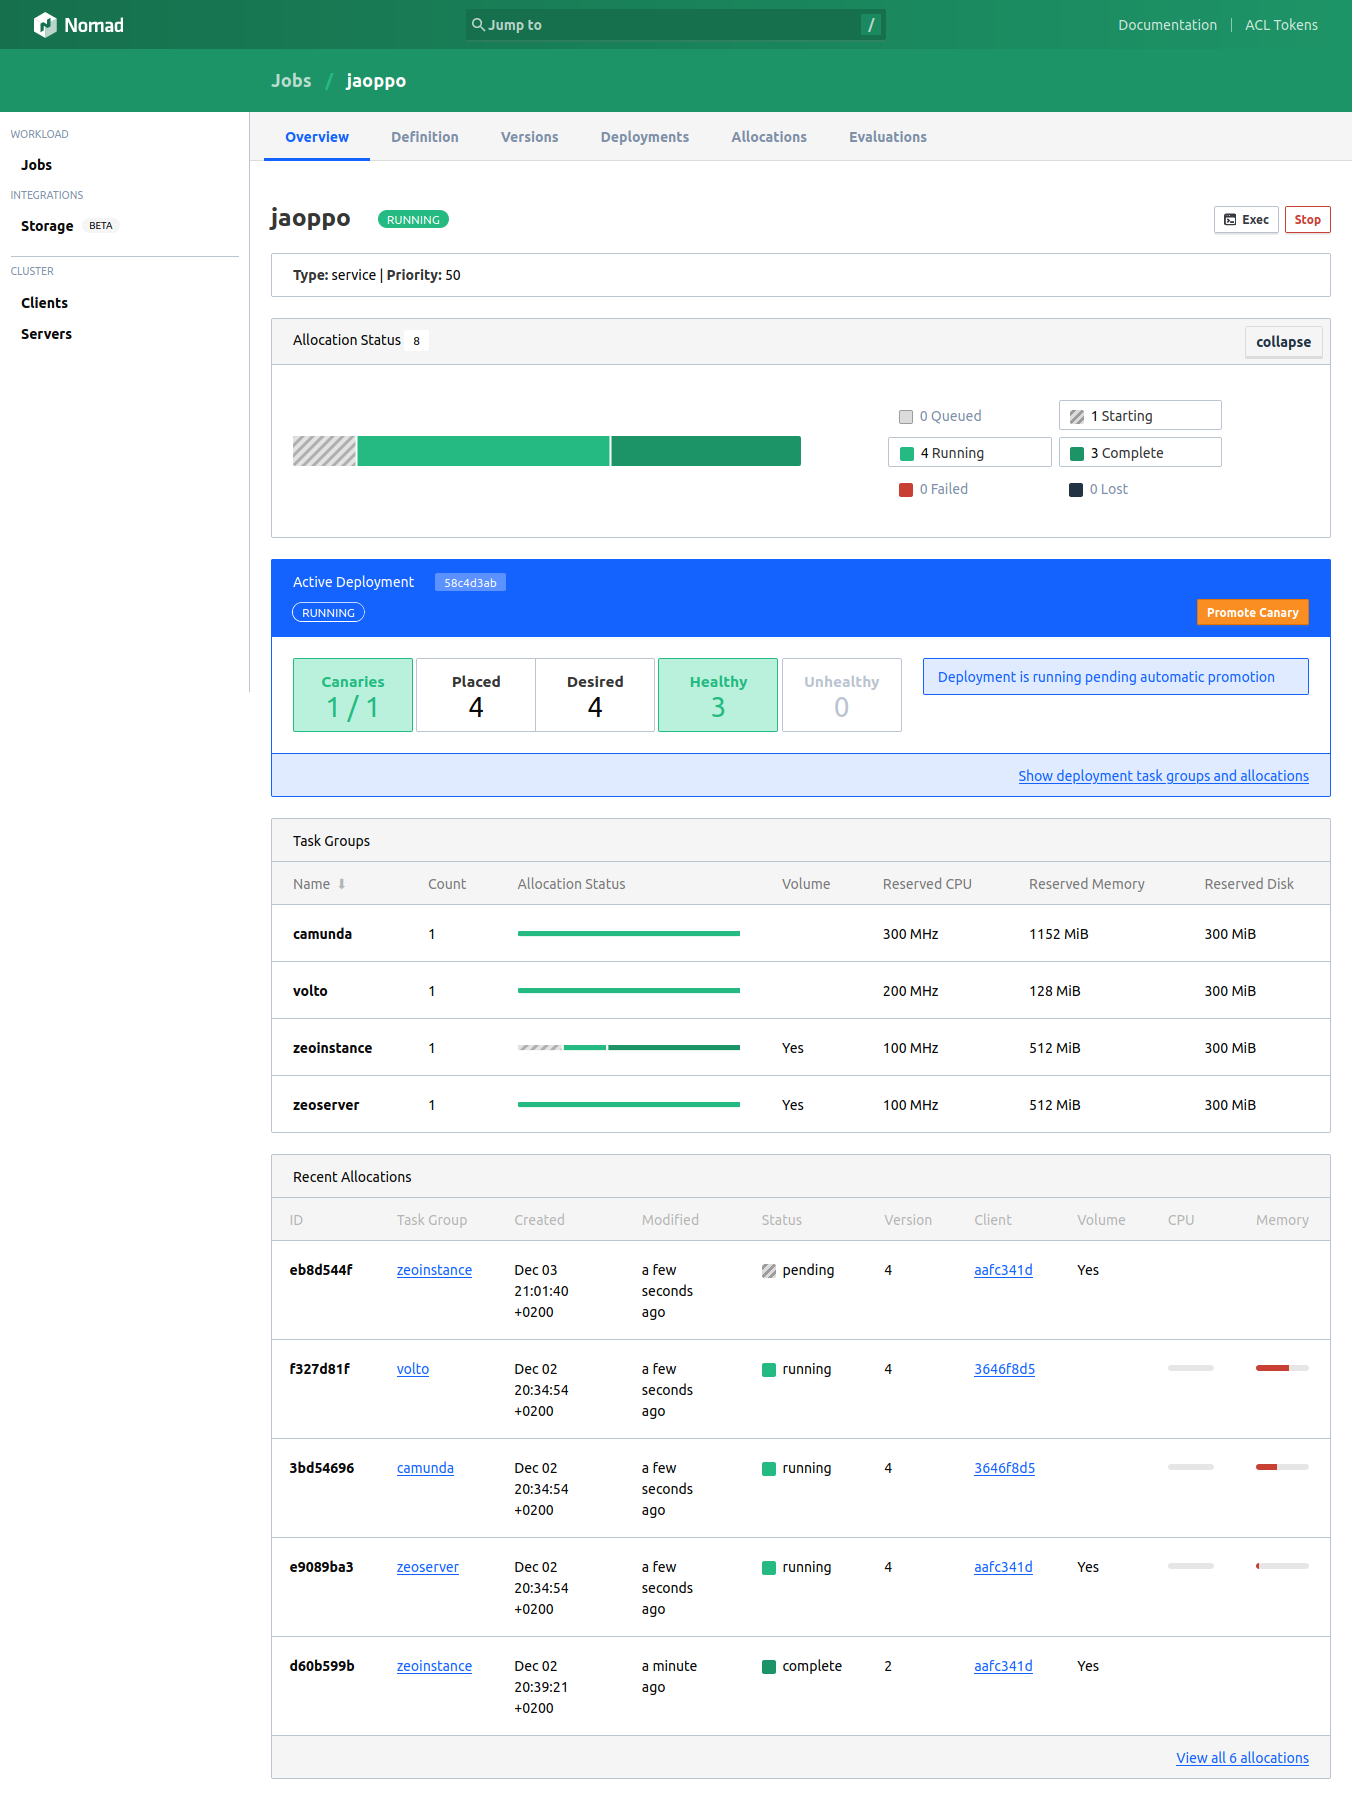
\includegraphics[height=1\paperheight]{images/nomad-02.png}
\columnbreak
~\par
~\par
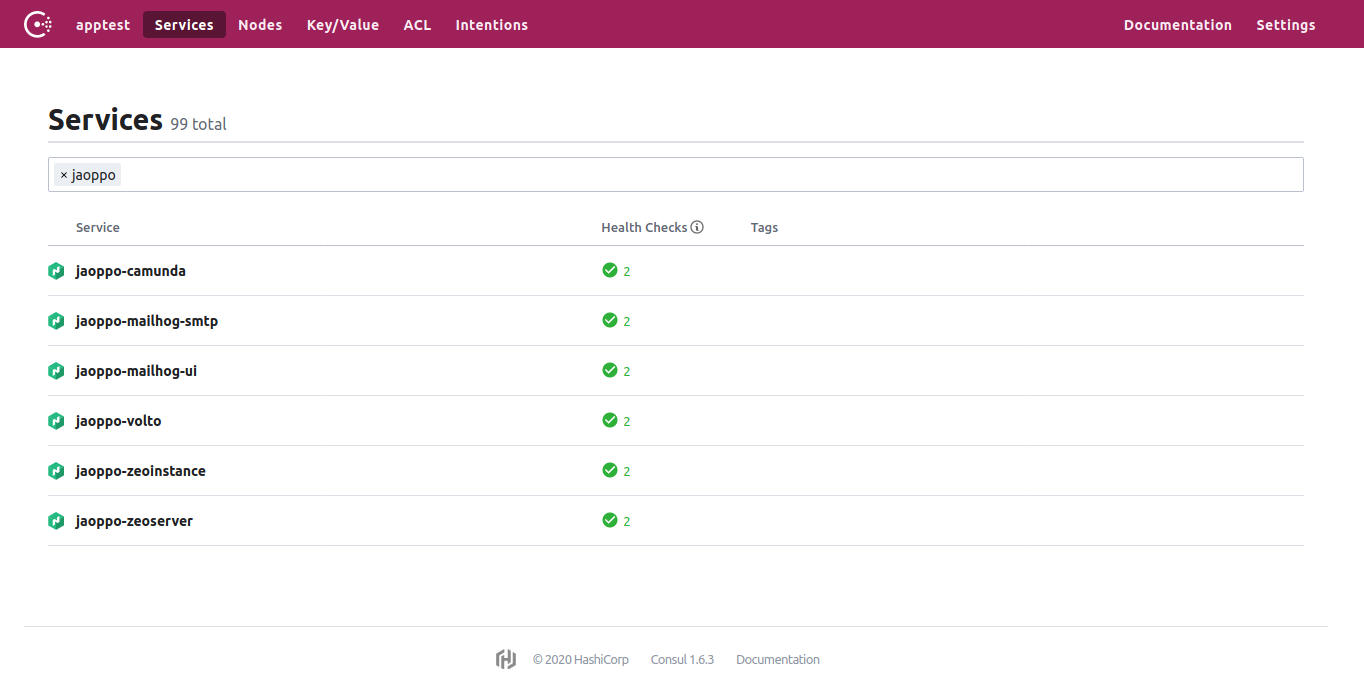
\includegraphics[width=0.45\paperwidth]{images/consul-01.png}
~\par
~\par
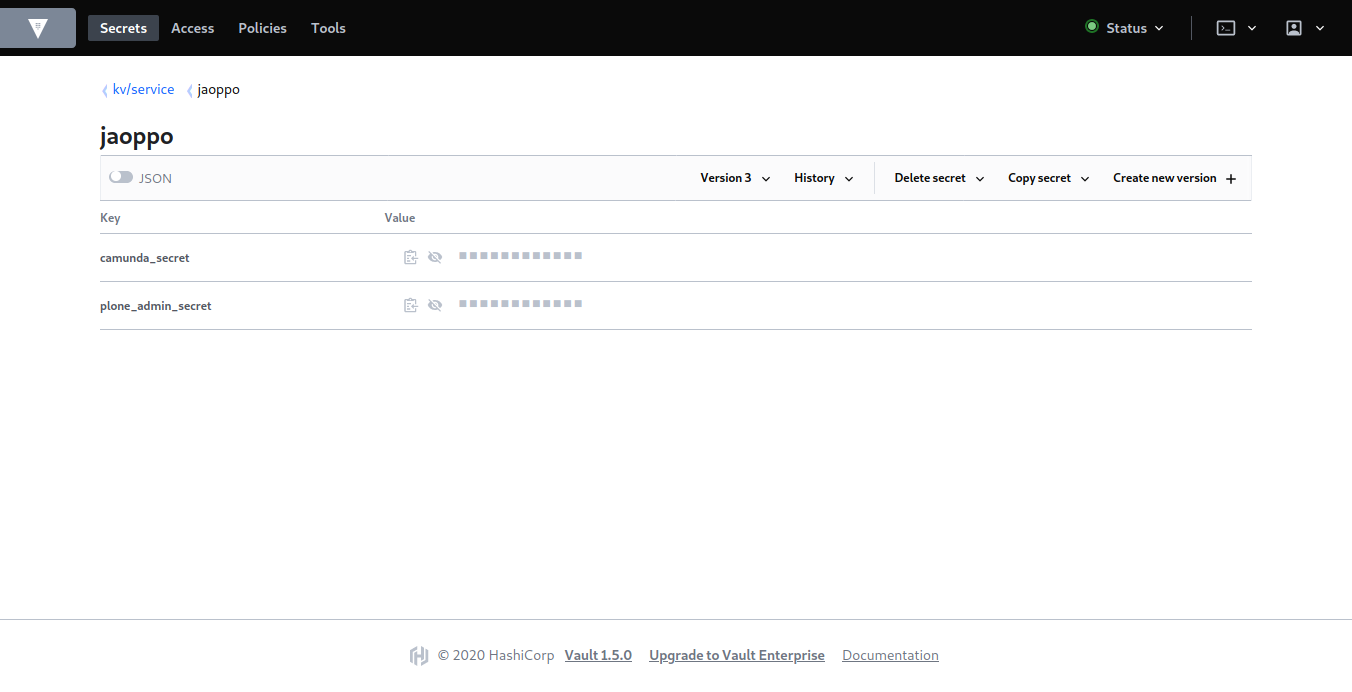
\includegraphics[width=0.45\paperwidth]{images/vault-01.png}
\end{multicols}
}
\end{frame}

%---------------------------------------------------------------------------------------

\setnomadtemplate
\begin{frame}{One Job File to Rule Them All}
  \begin{multicols}{3}
  \begin{itemize}
    \item task groups
    \item instance count
    \item update policy
    \item server resources
    \item volume mounts
    \item \ldots
    \item tasks
    \item consul services
    \item vault secrets
    \item env variables
    \item exec artifacts
    \item \ldots
    \columnbreak
  \end{itemize}
  \end{multicols}
\end{frame}

%---------------------------------------------------------------------------------------

\setnomadtemplate
\begin{frame}[fragile]{Nomad Isolated Fork/Exec Driver}
\textbf{Nix-built artifact}
\footnotesize
\begin{minted}{text}
artifact {
  source = "https://...app-[[ .app.version ]].tar.gz"
  destination = "/"
}
\end{minted}
\normalsize
\textbf{Runs on minimal chroot}
\footnotesize
\begin{minted}{text}
/etc/group
/etc/passwd
/etc/nsswitch.conf
/etc/resolv.conf
/etc/ssl/certs
\end{minted}
\end{frame}

%---------------------------------------------------------------------------------------

\setbeamertemplate{background canvas}[default]
\begin{frame}{}
\begin{picture}(0,0)(20,220)
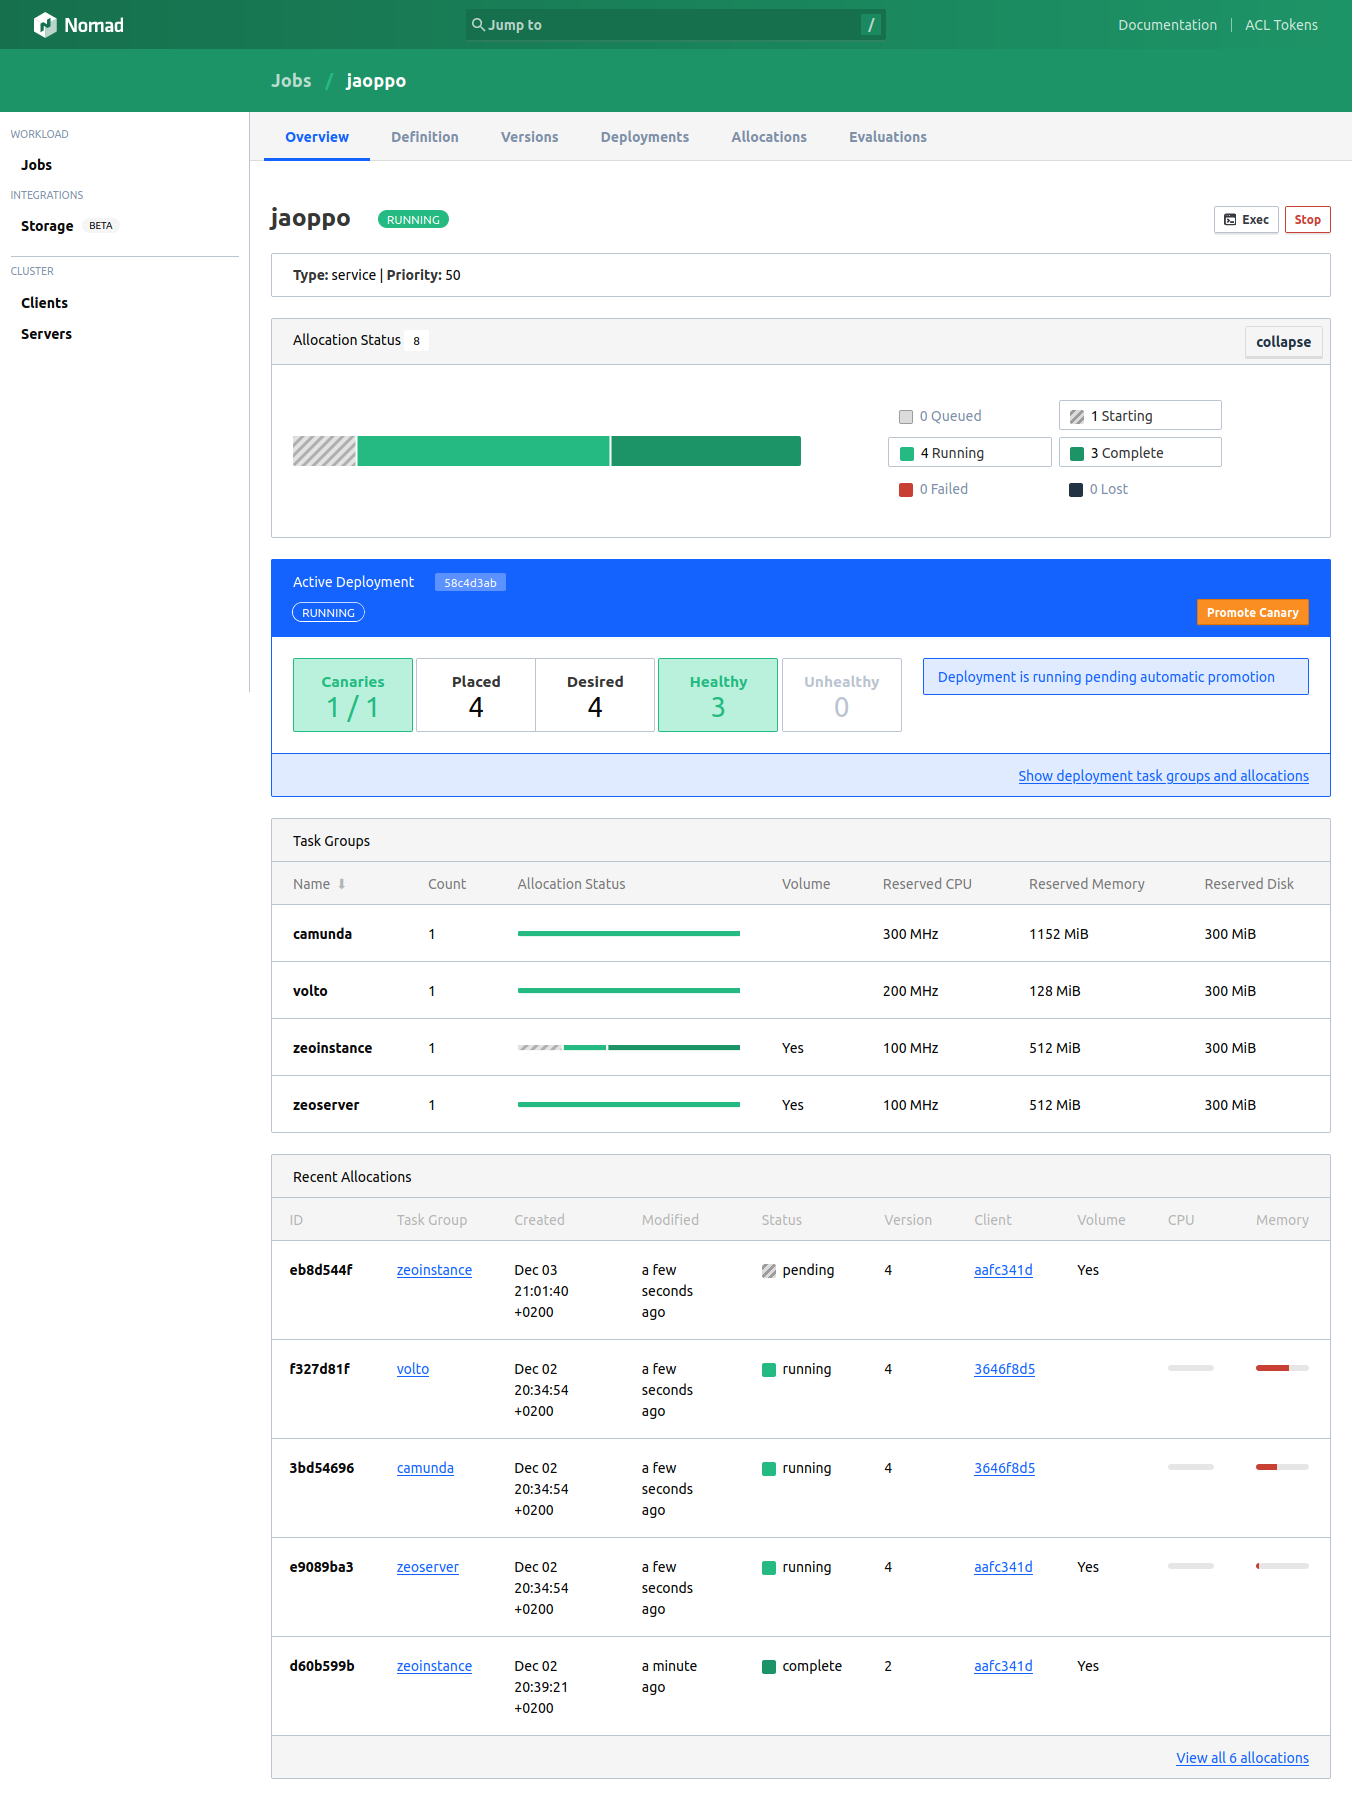
\includegraphics[width=0.8\paperwidth]{images/nomad-02.png}
\end{picture}
\end{frame}

%---------------------------------------------------------------------------------------

\setbeamertemplate{background canvas}[default]
\section{Nix-built Nomad artifacts}

%---------------------------------------------------------------------------------------

\setnixtemplate
\begin{frame}{One Package Manager to Rule Them All}
\textbf{Nix-built Nomad deployment artifacts}
\begin{multicols}{2}
  Advantages
  \begin{itemize}
    \item 100~\% reproducible
    \item production equals development
    \item sandboxed offline builds
    \item full dependency graph
    \item standalone tarballs
    \item no Dockerfile
    \item no base images
    \item no surprises
  \end{itemize}
  \columnbreak
  Disadvantages
  \begin{itemize}
    \item<1-> no conventions
    \item<1-> no metadata
    \item<1-> no shared layers
    \only<1>{\item<1-> no documentation}
    \only<2>{\item<1-> \sout{no documentation}}
    \item<2->[] \hspace{-2.2em} Some documentation
    \item<2-> https://nixos.org
    \item<2-> https://nix.dev
  \end{itemize}
\end{multicols}
\end{frame}

%---------------------------------------------------------------------------------------

\setnixtemplate
\begin{frame}[fragile]{\texttt{volto.tar.gz}}
\tiny
\begin{multicols}{2}
\begin{minted}{nix}
{ pkgs ? import ../nix { nixpkgs = sources."nixpkgs-20.09"; }
, sources ? import ../nix/sources.nix
, volto ? import ./default.nix { inherit pkgs; }
, name ? "artifact"
}:

with pkgs;

let

  env = buildEnv {
    name = "env";
    paths = [
      bashInteractive
      coreutils
      findutils
      gnused
      volto
    ];
  };

  closure = (writeReferencesToFile env);

in

runCommand name {
  buildInputs = [ makeWrapper ];
} ''
mkdir -p local/bin
makeWrapper ${bashInteractive}/bin/sh local/bin/sh \
  --prefix PATH : ${coreutils}/bin \
  --prefix PATH : ${volto}/bin \
  --prefix PATH : ${findutils}/bin \
  --prefix PATH : ${gnused}/bin \
  --prefix PATH : ${env}/bin
tar cvzhP \
  --hard-dereference \
  --exclude="${env}" \
  --exclude="*ncurses*/ncurses*/ncurses*" \
  --exclude="/nix/store/*-node_volto-starter-git*" \
  --files-from=${closure} \
  --transform="s|^local/||" \
  local > $out || true
''

\end{minted}
\end{multicols}
\end{frame}

%---------------------------------------------------------------------------------------

\setnixtemplate
\begin{frame}[fragile]{\texttt{/bin/volto}}
\tiny
\begin{multicols}{2}
\begin{minted}{nix}
pkgs.stdenv.mkDerivation {
  name = "volto";
  src = pkgs.lib.cleanSource ./.;
  builder = builtins.toFile "builder.sh" ''
    source $stdenv/setup;
    mkdir -p $out/bin $out/lib
    cp -a $src $out/lib/volto && chmod u+w -R $out/lib/volto
    cd $out/lib/volto
    cp -a $env node_modules
    HOST=CUSTOM_RAZZLE_SERVER_HOST \
    PORT=CUSTOM_RAZZLE_SERVER_PORT \
    RAZZLE_API_PATH=CUSTOM_RAZZLE_API_PATH \
    node_modules/.bin/razzle build
    chmod u+w -R node_modules && rm -r node_modules
    cat > $out/bin/volto << EOF
    #$bash/bin/env sh
    RUNTIME="\$(mktemp -d)"
    cp -R $out/lib/volto/build/* "\$RUNTIME"
    chmod u+w -R "\$RUNTIME"
    find "\$RUNTIME" -name "*.js"|xargs sed -i "s|CUSTOM_RAZZLE_SERVER_HOST|\$HOST|g"
    find "\$RUNTIME" -name "*.js"|xargs sed -i "s|CUSTOM_RAZZLE_SERVER_PORT|\$PORT|g"
    find "\$RUNTIME" -name "*.js"|xargs sed -i "s|CUSTOM_RAZZLE_API_PATH|\$RAZZLE_API_PATH|g"
    find "\$RUNTIME" -name "*.js"|xargs sed -i "s|$out/lib/volto/build|\$RUNTIME|g"
    chmod u-w -R "\$RUNTIME"
    cd $out/lib/volto && node "\$RUNTIME/server.js" $@
    EOF
    chmod u+x $out/bin/volto
    wrapProgram $out/bin/volto \
      --suffix PATH : $propagatedBuildInputs/bin \
      --suffix NODE_ENV : production \
      --suffix NODE_PATH : $env
  '';
  buildInputs = with pkgs; [ makeWrapper ];
  propagatedBuildInputs = with pkgs; [ nodejs-14_x ];
  inherit bash env;
}
\end{minted}
\end{multicols}
\end{frame}

%---------------------------------------------------------------------------------------

\setnixtemplate
\begin{frame}{Don't Try This at Home\textsuperscript{\faTrademark}}
  \textbf{Nix – the assorted ugly parts}
  \begin{itemize}
    \item every language has their own Nix-conventions
    \item Nix dependency generator ecosystem is complex
    \item Nix does not support cyclic dependencies
    \item no storage device is big enough for \texttt{/nix/store}
    \item many NPM packages want to call Internet on install
    \item some NPM packages ship with pre-built binaries
    \item \ldots
  \end{itemize}
\end{frame}

%---------------------------------------------------------------------------------------

\setbeamertemplate{background canvas}[default]
\section{Plone without buildout}

%---------------------------------------------------------------------------------------

\setmytemplate
\begin{frame}{Plone 5.2.1 without Buildout}
  \textbf{Our (legacy) approach for Plone with pip}
  \begin{itemize}
    \item generated requirements.txt with buildout
    \item created Python environment with pip / Nix
    \item used pip-branch of z3c.autoinclude
    \item disabled \texttt{<includeDependencies />}
    \item generated instance skeleton with Nix
    \item forked \texttt{plone.recipe.zope2instance} into \texttt{plonectl}
  \end{itemize}
\end{frame}

%---------------------------------------------------------------------------------------

\setnixtemplate
\begin{frame}[fragile]{\texttt{zope.conf}}
\tiny
\begin{multicols}{2}
\begin{minted}{nix}
{ pkgs ? import <nixpkgs> {}
, generators ? import ./generators.nix {}
, instancehome ? import ./instancehome.nix {}
, var ? "$(PLONE_VAR)"
}:

let configuration = generators.toZConfig {

 # ...

  zodb_db = {
    main = {
      cache-size = 40000;
      mount-point = "/";
      zeoclient = {
        read-only = false;
        read-only-fallback = false;
        blob-dir = "${var}/blobstorage";
        shared-blob-dir = true;
        server = "$(PLONE_ZEOSERVER_ADDRESS)";
        storage = 1;
        name = "zeostorage";
        var = "${var}";
        cache-size = "128MB";
      };
    };
    temporary = {
      temporarystorage = {
        name = "temporary storage for sessioning";
      };
      mount-point = "/temp_folder";
      container-class = "Products.TemporaryFolder.TemporaryContainer";
    };
  };
}; in

pkgs.stdenv.mkDerivation {
  name = "zope.conf";
  builder = builtins.toFile "builder.sh" ''
    source $stdenv/setup
    cat > $out << EOF
    $configuration
    EOF
  '';
  inherit configuration;
}
\end{minted}
\end{multicols}
\end{frame}

%---------------------------------------------------------------------------------------

\setnixtemplate
\begin{frame}[fragile]{\texttt{/bin/plonectl-zeoinstance}}
\tiny
\begin{minted}{nix}
  plonectl-zeoinstance = stdenv.mkDerivation {
    name = "plonectl-zeoinstance";
    zope_conf = import ./zconfig/zeoinstance.nix {};
    plonesite_py = ./zconfig/plonesite.py;
    builder = builtins.toFile "builder.sh" ''
      source $stdenv/setup
      mkdir -p $out/bin
      cat > $out/bin/plonectl-zeoinstance << EOF
      #!$bash/bin/sh
      mkdir -p \$PLONE_VAR/filestorage
      if [ ! -f \$PLONE_VAR/.sentinel ]; then
          $env/bin/python -m plonectl.cli instance -C $zope_conf run $plonesite_py
          touch \$PLONE_VAR/.sentinel
      fi
      $env/bin/python -m plonectl.cli instance -C $zope_conf \@$
      EOF
      chmod a+x $out/bin/plonectl-zeoinstance
    '';
    inherit bash env;
  };
\end{minted}
\end{frame}

\setmytemplate
\begin{frame}[fragile]{Plone 6 without Buildout}
  \begin{itemize}
    \item[\color{green}{\faCheck}] Plone 6 is pip installable (hearsay)
  \end{itemize}
  \begin{minted}{bash}
$ python3 -m venv py
$ ./py/bin/pip install Plone Paste -c ...
$ ./py/bin/mkwsgiinstance -d .
$ ./py/bin/runwsgi -v etc/zope.ini
  \end{minted}
  \begin{itemize}
    \item[\color{red}{\faTimes}] instance templates and scripts are still maintained \\ in \texttt{plone.recipe.zope2instance}
  \end{itemize}
\end{frame}

%---------------------------------------------------------------------------------------

\setmytemplate
\begin{frame}[fragile]{TxZServer in Production}
  \textbf{Plone 5.2.1 / Zope 4.1.3 / Twisted / WebSockets + ZMQ PubSub}
  \footnotesize
  \begin{minted}{cfg}
[sources]
ZServer =  git git@github.com:datakurre/ZServer
           branch=datakurre/master
collective.wsevents =
           git git@github.com:datakurre/collective.wsevents
plonectl = git git@github.com:datakurre/plonectl
  \end{minted}
  \begin{itemize}
    \item[\color{green}{\faCheck}] in production since March 2020 without known issues
    \item[\color{red}{\faTimes}] upgrade to Plone $>$ 5.2.1 and Zope $>$ 4.1 still pending
  \end{itemize}
\end{frame}

\setbeamertemplate{background canvas}[default]
\begin{frame}[standout]
\vfill

\includegraphics[height=0.50\paperheight]{images/plone-icon-hearts.png}
\par
\href{https://datakurre.github.io/ploneconf2020/alt}{datakurre.github.io/ploneconf2020/alt}
\end{frame}

%---------------------------------------------------------------------------------------

\end{document}
